

\documentclass{article}

% Packages

\usepackage[margin=1in]{geometry}
%\usepackage{graphicx}
%\usepackage{tikz-timing}
\usepackage{color}
\usepackage{commath}

\usepackage{setspace}
\doublespacing

\usepackage{cite}
\usepackage{caption}
\usepackage{subcaption}
\usepackage{hyperref}
\usepackage{listings}

% Automatix LaTeX build system modules

%\usepackage{svg}
%\usepackage{mat}
\usepackage[dvipdfm]{graphicx} 
\usepackage{bmpsize}

\usepackage{subfig}
\usepackage{tabularx}

%[stevo]: specify location of images here
%\usepackage{graphicx}
% declare the path(s) where your graphic files are
\graphicspath{{images/}}
% and their extensions so you won't have to specify these with
% every instance of \includegraphics
\DeclareGraphicsExtensions{.pdf,.jpeg,.png}

\newcommand{\degree}{\ensuremath{^\circ}}
% Now we actually start the document

\begin{document}

% Note that we are defining both the title and the author -- LaTeX will decide where
% they ought to go in the final typeset, depending on the style we've selected.

\title{ASTRO 121: Lab 3  \\ \normalsize Radio Interferometry at X Band}

\author{Rachel Hochman}


% The \markboth command simply determines how the pages will be marked.
% There are two arguments, since for double-sided pages, you often want a different
% marking on facing pages.

%\markboth{Team DarkStar, ASTRO121, Spring 2015}{Team DarkStar, ASTRO121, Spring 2015}

%Now we tell Latex to create the title, based on the info we've provided.

\maketitle


\section{Introduction}

The first goal of this lab was to learn about 'fringes.' We first explored how diffraction theory applies to an actual radio interferometer, and what the resulting fringe looks like in terms of its amplitude and phase. Once we obtained the fringe, we explored its properties further by taking a Fourier transform and Fourier filtering the fringe. We practiced these techniques on data taken of the Sun, and then we also obtained data of the Moon and a point source- M17 in our case. The other main goal of this lab was to expand on our knowledge of least-squares fitting techniques, specifically learning how to do \textit{nonlinear} least-squares fitting. Finally, we explored the Fourier transform relationship between interferometer response and sky brightness by using nonlinear least-squares fitting to obtain accurate diameters for the Sun and Moon.

\section{Experimental Setup}

All data collection for this lab was done with a multiplying interferometer.  The interferometer consists of two receiver dishes, each with a series of filters and mixers, as shown in \autoref{fig:interf}.  The received signal goes through a low power amplifier, a bandpass filter, a low noise amplifier, and a mixer within the feed of the dish. The signal is then brought into the lab where it goes through second bandpass filter, the second mixer, and a third bandpass filter. Finally the two signals from each side are mixed together in a DSB mixer.

An interferometer is desired over a single radio antenna because of increased angular resolution. Whereas the angular resolution of a single antenna with diameter \textit{D} is proportional to $\lambda/D$, the angular resolution achieved by two dishes separated by a baseline \textit{B} is proportional to $\lambda/B$. Consequently, the farther the two dishes are separated, the better the angular resolution.

\begin{figure}[h!]
 \begin{center}
    \includegraphics[width=5in, angle=90]{interf.ps}
    \caption{\bf{Interferometer Diagram}}
    \label{fig:interf}
     \end{center}
    \end{figure}
\newpage

The output of the interferometer is a sinusoidal-like signal called the "fringe."  Given a known baseline \textit{$B_y$} and the frequency, phase, and amplitude properties of the fringe, we can measure the declination of a point source as well as the diameters of the Sun and Moon. Exactly how will be discussed in later sections.

\subsection{Data Collection}
I wrote a script to take interferometry data, which uses the IDL procedures \texttt{isun} or \texttt{imoon} to calculate an altitude and azimuth for the object of interest. Additionally, I wrote a separate script which calculates these values using rotation matrices and double checked that each script gave the same outputs. Right ascension and declination values for the point sources came from the J2000 equinox, and therefore needed to be precessed to the current equinox. These values were then converted to local altitude and azimuth values using the local sidereal time (LST) and Campbell Hall's latitude and longitude. 
The tracking script updates the values every 10 seconds, using the \texttt{point2} command to set the orientation of the dishes. It also re-calibrates the dishes about every hour using the \texttt{homer} command, in case the dishes lose alignment.

\subsection{Choice of Mixing Frequency}

Initially, each lab group was to chose an L.O. frequency of 11.3,11.5,11.7,11.9,12.1, and 12.3 GHz. My group's initial Sun data was taken with the first L.O. frequency set to 12.3GHz. However, we later realized when looking at the initial filter with a passband of 10-18 GHz, that the maximum frequency we should have been using was 11.7GHz. This is because the later bandpass filter narrowly selects for 1.7 GHz, meaning that the frequencies we are actually recording from the sky are L.O.1 $\pm$ 1.7 GHz. Therefore, for any L.O. frequency above 11.7 GHz, such as 12.3 GHz, both frequencies are within the passband (in this case 10.6 GHz and 14 GHz). Choosing an L.O.1 of 11.3 GHz however, would mean that we would see 9.6 GHz and 13 GHz. However, the 9.6 GHz component would have been filtered out by the first bandpass filter, leaving only the 13 GHz component.

Since we used 12.3 GHz for our sun data, we use the $\lambda$ which corresponds to 10.6 GHz, and for the data taken with 11.7 GHZ as the L.O.1 frequency we use the $\lambda$ corresponding to 10 GHz.

\subsection{Dish Accuracy}

When tracking the Sun, we attempted to visually confirm that the dishes were pointing directly at the Sun by checking that the feed shadow lined up directly with the center of the dish. In reality, the shadows did not line up perfectly, but were generally 1-3cm way from the center. Given a 1 meter distance from the feed to the dish, this means that the the dishes were up to 1.7\degree off from the desired position. For extended sources such as the sun, this offset can reduce the fringe amplitude but otherwise has no huge effects. For point sources, however, this offset reduces the chances of pointing directly at the object, and possibly prevents the dishes from pointing at the object at all. Additionally, we noticed that sometimes the wind atop Campbell Hall was strong enough to shake the dishes by several degrees, reducing the accuracy even further.

\section{The Fringe}
Because we use two different dishes separated by baseline \textit{$B_y$}, there is a difference in their distances from the source. This difference is distance is made up of the geometrical path delay $\tau_{g}$ as well as any difference in cable length $\tau_{c}$. We know $\tau_{g}$, which is a function of the hour angle of the source ($h_s$), from the geometry of the interferometer. For the east-west baseline we have:

\singlespacing
\begin{eqnarray}
 \tau_{g}(h_s) =\bigg[ \frac{B_y}{c}cos\;\delta \bigg] sin\;h_s
\end{eqnarray}

Therefore, the voltages for the two telescopes looking at a monochromatic source are: 

%\singlespacing
\begin{eqnarray}
 E_1(t) =cos(2\pi\nu t) \\
 E_2(t) =cos(2\pi\nu \big[ t+\tau_{tot}\big])
\end{eqnarray}
%\doublespacing

and the product is the interferometer fringe output:

\begin{eqnarray}
 F(t) =cos(2\pi\nu t) cos(2\pi\nu \big[ t+\tau_{tot}\big])
\end{eqnarray}
\doublespacing
Using various trig identities and the fact that $\frac{\nu}{c} = \lambda$ (see handout for each individual step) we are left with the fringe amplitude for a point source:


\begin{eqnarray}
 F(h_s) =Acos\bigg[ 2\pi(\frac{B_y}{c}cos\;\delta)sin\;h_s \bigg] -Bsin\bigg[ 2\pi(\frac{B_y}{c}cos\;\delta)sin\;h_s \bigg]
\label{eq:lss}
\end{eqnarray}

where  $A = cos(2\pi\nu\tau_c)$ and $B = sin(2\pi\nu\tau_c)$. Looking at the argument inside the cosine and sine in each term, we see a constant $C = \bigg[2\pi( \frac{B_y}{c}cos\;\delta )\bigg]$ multiplied by $sin(h_s)$. Because $h_s$ is the hour angle and increases monotonically with time, we can regard it as time. Therefore, the product $C sin(h_s)$ is the argument of the cosine terms and makes it oscillate with a with a frequency that depends on time. 

If you expand the hour angle term $sin(h_s)$ into a Taylor series, and consider that $F(h)$ varies as $f_f \;\Delta h$, you end up with a local fringe frequency of:

\begin{eqnarray}
f_f = \frac{C}{2\pi}cos(h_s)= \bigg(\frac{B_y}{\lambda}cos\delta \bigg) cos(h_s)
\label{eq:ff}
\end{eqnarray}
This value is in cycles per radian on the sky. To convert into cycles per minute, you must multiply by $\frac{2\pi}{60\times24}$ and to get cycles per second by $\frac{2\pi}{60\times60\times24}$.

\section{The Sun}
 
We began by taking fringe data of the Sun on March 12th using an L.O.1 of 12.3 GHz. \autoref{fig:fringe} shows the Sun fringe data with all 9 hours of data gathered as well as a zoomed in version.


\begin{figure}
        \centering
        \begin{subfigure}[b]{\textwidth}
                \centering
                \includegraphics[width=6in]{sun_fringe.ps}
                \caption{}
                \label{fig:fringeout}
        \end{subfigure}%
        \newline
        \begin{subfigure}[b]{\textwidth}
        	       \centering
                \includegraphics[width=6in]{sun_fringe_zoom.ps}
                \caption{}
                \label{fig:fringezoom}
        \end{subfigure}


        \caption{Sun Fringe Data. Subfigure (a) contains the entire 9 hours of data taken, and subfigure (b) shows a zoomed in version to highlight the sinusoidal nature of the fringe pattern.}\label{fig:fringe}
\end{figure}


A valuable exercise was to use the above 'local fringe frequency' equation to predict what frequencies we would see in the sun data, and then to confirm this by taking a Fourier transform of the Sun data. I performed the following calculations only on the first three hour chunk of sun data for simplicity (and because while we were observing the sun later, there was an attempt by another group to control the dishes and this might have corrupted the data). Our first set of Sun data was taken between the hour angles of -3 and 0. Therefore, the values of $cos(h_s)$ should range from $cos(-3\times 15)$ to $cos(0)$, or .707-1. Therefore, given a $B_y$ of 1524 cm and a $\lambda$ of 2.83 cm, a declination of $\lambda\approx0$ since this data was taken almost at the equinox, and substituting into \autoref{eq:ff} we expect to see a range of frequencies from .0277Hz to .0392Hz.

Indeed, taking the Fourier transform of the Sun fringe data results in \autoref{fig:sun_dft}, which shows that there are frequency components roughly between .027 and .039Hz. The reason there is more power at the higher end (.039Hz) is because this is the so-called 'transit' frequency, when the Sun is directly overhead, and spends a longer time at this frequency.


\begin{figure}[h!]
 \begin{center}
    \includegraphics[width=6.5in]{sun_dft.ps}
    \caption{\bf{Sun DFT}}
    \label{fig:sun_dft}
     \end{center}
    \end{figure}
    
    
\section{Non-Linear Least Squares Fitting}

The least-squares fitting technique was used on \autoref{eq:lss}, and was done as follows. First we treat the entire value of $\bigg[ \frac{B_y}{\lambda}cos\;\delta \bigg]$ as an unknown, \textit{C}, and adopt a value for the right ascension $\alpha$ to compute $h_s$. Given these assumptions, we use the standard least-squares process to solve for the values of \textit{A} and \textit{B}. The least-squares process we used was the \texttt{CURVEFIT} function in IDL. We then sweep through different values of C and save the value of the sum of the residuals squared for each value. The value of C that gives the minimum sum-of-squares is the best value of C. The code that performed this is given below. 

\lstset{basicstyle=\footnotesize}


\begin{lstlisting}[frame=single]
;the function called 'fringe' is F = A[0]*cos(C*sin(x)) - A[1]*sin(C*sin(x))
;the 'answer' F is the array of voltage values gathered
F = volts
;here we calculate the hour angle
X = lst - ra ; hour angle is lst-ra
X = X*15*(!dpi/180.0) ; make it into radians
;make a blank array that has two values (A and B in our case)
pointz = make_array(2, stopval-startval, /double)
startval = 3000l
stopval = 5000l
A = [0.5, 0.5] ;initial guess for A
for jj=startval, stopval-1 do begin ; sweep through different values of C
      common share, c
      c = jj
      fit = CURVEFIT(X, F, weights, A, function_name = 'fringe', /noderivative, CHISQ=ressq)
      print,jj
      pointz[0,jj-startval] = jj ;assign value of C to the 1st elem in the array
      pointz[1,jj-startval] = ressq ; assign the sum of the squares of residuals to 2nd elem

\end{lstlisting}

This is the so-called 'brute-force' technique using least-squares. There is a more elegant way of computing the least squares but it only gives local minima, meaning you have to put the initial guess extremely close to the real answer or you could end up with the wrong minimum. Therefore we stuck to using this brute-force method.

In addition we solve for $C = \bigg[2\pi( \frac{B_y}{c}cos\;\delta )\bigg]$ rather than simply $cos\;\delta$ because if we use a baseline that is too small in the solution, the best value for $cos\;\delta$ maybe larger than unity- meaning that no declination will give a satisfactory solution! INstead we solve for C and derive the declination from that value.

We then plot the values of the sum-of-squares versus the value of $C$ in \autoref{fig:ls_sun}. The lowest minimum in the resulting plot is at $C=3354$. Since $C = \bigg[2\pi( \frac{B_y}{c}cos\;\delta )\bigg]$, we can calculate backwards and find that $cos\; \delta = .9915$, or $\delta\approx7^\circ$which is extremely close to our expected value of $cos\;\delta=.9983$, or $\delta\approx3^\circ$. This expected value comes from looking up the declination of the sun on March 12 here: http://www.wsanford.com/\~{}wsanford/exo/sundials/DEC\_Sun.html.

\begin{figure}[h!]
 \begin{center}
    \includegraphics[width=6in]{LS.ps}
    \caption{\bf{Least Squares Fitting of Sun Data}}
    \label{fig:ls_sun}
     \end{center}
    \end{figure}
    
    
\section{The Moon}

The same process was repeated for the Moon. Unfortunately, our group did not collect any good Moon data, so Team BADWOLF was kind enough to let us use their raw Moon data collected on March 17th with and L.O.1 of 11.7 GHz.  \autoref{fig:moon} is a plot of raw Moon data versus hour angle (calculated by LST-RA).

\begin{figure}[h!]
 \begin{center}
    \includegraphics[width=5.5in]{moon_data.ps}
    \caption{\bf{Moon Data}}
    \label{fig:moon}
     \end{center}
    \end{figure}

\autoref{fig:moon_dft} shows the Fourier transform of the Moon Data. Using \autoref{eq:ff} again and given $\lambda=3 cm$ and $\delta \approx -12^\circ$, we can calculate that the expected values of $f_f$ for hour angles of -4 to 0 is .0181 Hz to .0361 Hz. There is a significant bump within that range, again with more power at the upper frequency value, since that corresponds to the transit frequency. It is not quite as well-defined as the Sun data, but very close.

\begin{figure}[h!]
 \begin{center}
    \includegraphics[width=5.5in]{moon_dft.ps}
    \caption{\bf{Moon DFT}}
    \label{fig:moon_dft}
     \end{center}
    \end{figure}
  
\autoref{fig:ls_moon} is the Least Squares Fitting results for the Moon Data.  Again I plotted the values of the sum-of-squares versus the value of $C$ and found that the lowest minimum in the resulting plot is at $C=3156$. Calculating backwards we get that $cos\; \delta = .9888$ or $\delta\approx9^\circ$, which is somewhat close to our expected value of $cos\;\delta=.9781$ or $\delta\approx12^\circ$
    
\begin{figure}[h!]
 \begin{center}
    \includegraphics[width=5.5in]{moon_fit.ps}
    \caption{\bf{Least Squares Fitting of Moon Data}}
    \label{fig:ls_moon}
     \end{center}
    \end{figure}


\section{Point Source Data} 
As with the Moon data, our team did not collect any reasonable point source data, so we borrowed M17 data from Team BADWOLF, which they collected data on March 8, using an L.O.1 of 11.7 GHz. Since the procedure is the same as that of the Sun and Moon, most steps will be omitted here. NB: All Figures in this section were made by Stevo Bailey. 

\autoref{fig:m17_time} shows the time-series fringe data from M17. Since the signal of the point source is very weak and contains noise, the time-series does not look strongly sinusoidal. 
Next, the Fourier transform was taken to view the fringe spectrum. The expected frequency range was calculated using \autoref{eq:ff} above and found to be .026 Hz to .0475 Hz. However, the spectrum shown in \autoref{fig:m17_dft} shows lots of low-frequency components, but nothing that resembles a fringe, which hints at more problems with the data.

To find the declination, linear least-squares fitting on \autoref{eq:lss} was done, and the results are shown in \autoref{fig:m17_fit}. Note here the minimum is much shallower than before, suggesting the results may be inaccurate or due to noise. The minimum occurs at C = 3377.4, and for this C value, the declination is $37.84^\circ$, which is over $16^\circ$ from the expected value of $16.17^\circ$. Again this suggests problems with the data.



\begin{figure}
\begin{center}
\includegraphics[width=\linewidth]{m17_time.eps}
\caption{\bf{Time-series fringe data of M17, collected March 8, 2015}}
\label{fig:m17_time}
\end{center}
\end{figure}

\begin{figure}
\begin{center}
\includegraphics[width=6in]{m17_dft.eps}
\caption{\bf{DFT of the M17 fringe data}}
\label{fig:m17_dft}
\end{center}
\end{figure}

\begin{figure}
\begin{center}
\includegraphics[width=6in]{m17_fit.ps}
\caption{\bf{Linear least-squares fitting result on M17 data}}
\label{fig:m17_fit}
\end{center}
\end{figure}



\section{Diameter of Sun and Moon}   

Interferometer Response for a non-point-source object such as the Sun or Moon is given by:

\begin{eqnarray}
R(h_s) = F(h_s) \times \int  I(\Delta h) cos(2\pi f_f \Delta h) d\Delta h\
\label{eq:Rhs}
\end{eqnarray}

Where the first term is the known as the point-source fringe and the second term is the 'fringe modulator.' Generally, the modulating function is the Fourier transform of the source intensity distribution on the sky. For the flat distribution of the modulating function, the response can and does go through zero, and these zeros occur for $f_f = \frac{n}{2R}$. If we substitute into \autoref{eq:ff}  we have:

\begin{eqnarray}
 \bigg(\frac{B_y}{\lambda}cos\delta \bigg) cos(h_s) = \frac{n}{2R}
\label{eq:ff_radius}
\end{eqnarray}


To solve for R, we picked a zero at hour angle = -2.2474. With a $B_y$ of 11.6955 and $\lambda = 2.56 cm$, and sweeping values of $n$ through 4,5, and 6, we get the angular diameter of the moon is 0.008766 radians, which is close to the known value of 0.0088 radians or $\approx$.5 degrees. The Sun has roughly the same angular diameter when viewed from the Earth, and we calculated a value of $\approx$ 0.009 radians for the Sun as well.

\section{Conclusion and Acknowledgments}

In this lab we observed the fringes from the Sun,  the Moon, and M17. From this raw data we were able to take Fourier transforms to gain knowledge of the frequency components present in the fringe, and do a least squares fitting to obtain best values for the declination of each. Finally, using this information we were able to very accurately calculate the diameters of the Sun and Moon. 

%\section{Acknowledgements and Notes}
Thanks as always to Professor Carl Heiles and Katherine DeKleer for their help. Thanks also to the other members of Team Darkstar: Stevo Bailey, Brianna Grado-White, and Mahrud Sayrafi. Thanks this week to Team BADWOLF, for sharing their raw data with us.



\end{document}


--------------------------------------------------------------------------------
